\documentclass{../puzzlehunt}
\usetikzlibrary{calc,shapes,patterns,arrows}

\usepackage[puttinydots]{braille}
\usepackage{multicol}

\phSetTitle{MaPP Challenge '19 -- To Aleph-Zero And Beyond}
\phSetAuthor{Mathematical Puzzle Programs}
% \phUseAuthorWithTitle

%\phMarkDraft % comment out to remove draft watermark
\phShowPageNumbers % comment out to hide page numbers

% replace these with your image files
\phSetBannerLogo{mapp-banner}
\phSetSquareLogo{mapp-square}

\newcommand{\escapeKenKenLevel}[3]{
  \begin{scope}[shift={#1}]
    \fill[white] (0,0) rectangle (4,4);
    \draw[black!40,step=1,dashed] (0,0) grid (4,4);
    \draw[thick] (0,0) rectangle (4,4);
%    \node[anchor=south] at (2,4) {Level #2};
%    % \node[anchor=east] at (-0.3,2) {\rotatebox{90}{Rows}};
%    \node[anchor=east] at (0,0.5) {A};
%    \node[anchor=east] at (0,1.5) {B};
%    \node[anchor=east] at (0,2.5) {C};
%    \node[anchor=east] at (0,3.5) {D};
%    % \node[anchor=north] at (2,-0.3) {Columns};
%    \node[anchor=north] at (0.5,0) {A};
%    \node[anchor=north] at (1.5,0) {B};
%    \node[anchor=north] at (2.5,0) {C};
%    \node[anchor=north] at (3.5,0) {D};
    #3
  \end{scope}
}
\newcommand{\escapeKenKenUp}[1]{
  \node[anchor=south west] at #1 {\textcolor{black!60}{\footnotesize\(\uparrow\)}};
}
\newcommand{\escapeKenKenDown}[1]{
  \node[anchor=south east] at ($#1+(1,0)$) {\textcolor{black!60}{\footnotesize\(\downarrow\)}};
}
\newcommand{\escapeKenKenEasy}[2]{
  \node[blue] at ($#1+(0.5,0.5)$) {#2};
}
\newcommand{\escapeKenKenHard}[2]{
  \node[blue] at ($#1+(0.5,0.5)$) {#2};
}



\begin{document}

%\phTitlePage % Prints title page.
%\phTableOfContents % Prints table of contents

\phChapterWorksheet{Game Resources}{South Alabama Campus Map}

\begin{center}
  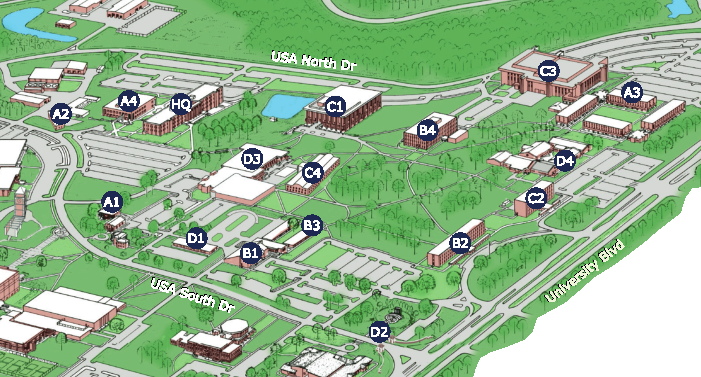
\includegraphics[width=\linewidth]{south-map}
\end{center}

\begin{multicols}{2}
  \begin{itemize}
    \item A1: Alumni Hall
    \item A2: Archaeology Museum
%    \item Central Services Admin Building % 30.69875, -88.17618
    \item A3: Charles M. Baugh Biomedical Library
    \item A4: Chemistry Building
    \item B1: Computer Services Center
    \item B2: F.P. Whiddon Administration Building % 30.6954, -88.17492
%    \item Glass Arts Building % 30.69708, -88.17642
%    \item Humanities Building
    \item B3: Innovation in Learning Center
    \item B4: Life Sciences Building
    \item C1: Marx Library
    \item C2: Math. Sciences and Physics Bldg. 
    \item C3: Medical Sciences Building
    \item C4: Meisler Hall % 30.69595, -88.17747
%    \item Mobile Townhouse 
    \item D1: Student Health Center
    \item D2: Tholos of Delphi Replica
    \item D3: USA Student Center
    \item D4: Visual Arts Complex
  \end{itemize}
\end{multicols}

Team Headquarters are located in the Humanities
Building (labeled HQ on the map).
Players will not need to cross USA South Dr, USA North Dr, or University Blvd.
\end{document}
